\documentclass[aspectratio=169]{beamer}

\usepackage{makecell}
\usepackage{booktabs}

\usetheme{Boadilla}
\setbeamertemplate{navigation symbols}{}

\title{Epidemic Broadcast}
\subtitle{Performance Evaluation of Computer Systems and Networks}
\author[Abdulwahed, Cima, Scatena]{Ahmed Khalil A. Abdulwahed, Lorenzo Cima, Niccolò Scatena}
\institute[UNIPI]{University of Pisa}
\date{2020/2021}

\begin{document}

\begin{frame}
	\titlepage{}
\end{frame}

\section{Simulation model}

\begin{frame}{The model}
	\begin{columns}
		\column{0.6\textwidth}
		\begin{itemize}
			\item 2D floorplan with users randomly dropped in
			\item A random user sends out a message; the other users
				relay it with a broadcast radius \emph{R}
			\item Time is \emph{slotted}
			\item \textbf{Trickle relaying}: when a user receives a
				message, it waits for \(T\) slots: message
				relayed if less than \(m\) copies received
		\end{itemize}
		\column{0.35\textwidth}
		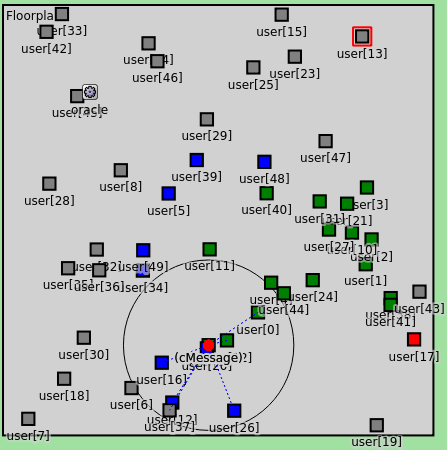
\includegraphics[width=\textwidth]{img/snapshot}
	\end{columns}
	Modules:
	\begin{description}
		\item[Floorplan] the network representing the 2D
			floorplan
		\item[User] submodule representing a user
		\item[Oracle] used to terminate simulation and collect
			some stats
	\end{description}
\end{frame}

\begin{frame}{User module}
	\begin{columns}
		\column{0.5\textwidth}
		Finite State Machine
		\begin{description}
			\item[IDLE] state when started; slotting through
				self-messages
			\item[RECEIVING] hearing message in current slot
			\item[COLLISION] received another message in the same
				slot
			\item[HEARING] waiting for time window \(T\)
			\item[RELAYING] relay message if trickle relaying not
				triggered
		\end{description}
		\column{0.5\textwidth}
		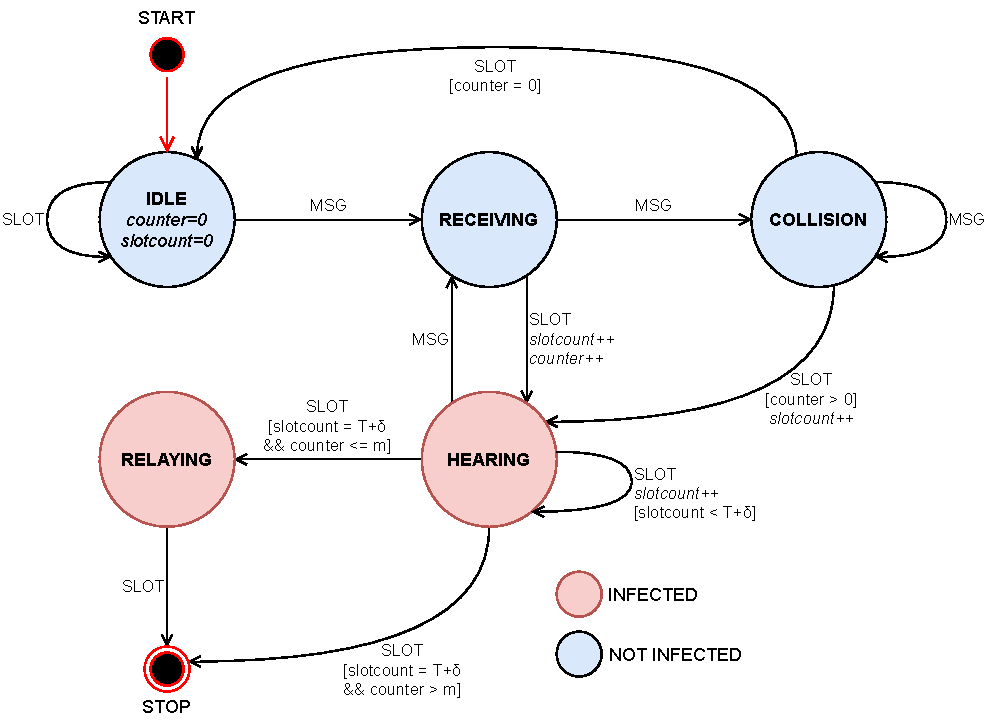
\includegraphics[width=\textwidth]{img/userfsm}
	\end{columns}
	User messages are sent with a duration equal to
	\(\frac{slotDuration}{2}\) in order to ensure that it is
	received in current slot
\end{frame}

\begin{frame}{Model verification}
	\begin{columns}
		\column{0.5\textwidth}
		\begin{description}
			\item[Valgrind] no memory leaks
			\item[Graphical] execution inside QTEnv
			\item[Step-by-Step Debug] check that the correct code
				execution path is taken
			\item[Event Trace] check for correct scheduling of
				events
			\item[Deterministic] same inputs \textrightarrow{} same
				outputs
			\item[Degeneracy] config with low params values
			\item[Continuity] little input change \textrightarrow{}
				little output change (figure)
		\end{description}
		\column{0.5\textwidth}
		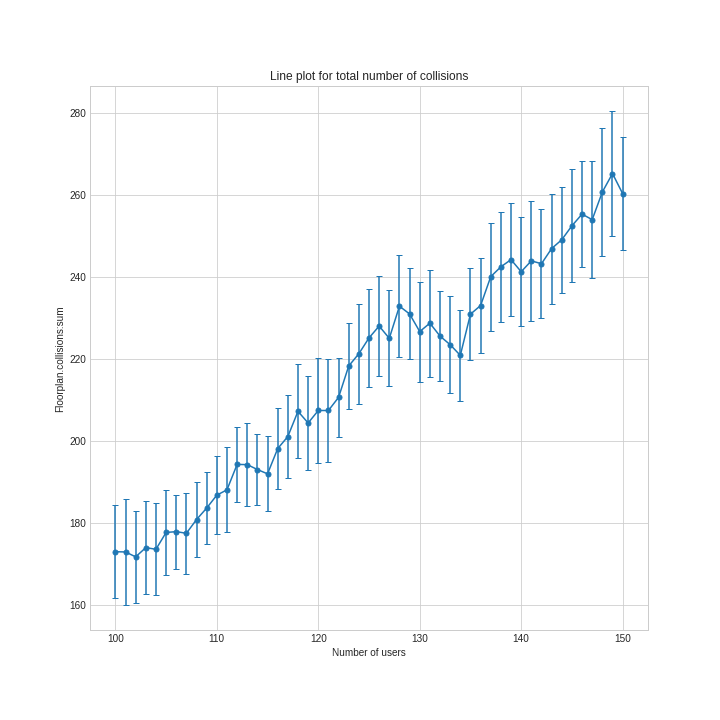
\includegraphics[width=\textwidth]{img/continuity-collisions}
	\end{columns}
\end{frame}

\section{Experiments design}

\begin{frame}{Factors and Indexes}
	\begin{columns}
		\column{0.5\textwidth}
		Performance indexes:
		\begin{itemize}
			\item \textbf{Broadcast time} needed to cover a certain
				percentile of the users
			\item Final percentage of \textbf{covered users}
			\item \textbf{Energy efficiency}: depends on \(R\) and
				the number of messages sent
				\[\mathit{Eff} \propto \frac{1}{R \cdot M}\]
			\item \textbf{Collisions}
		\end{itemize}
		\column{0.5\textwidth}
		Tunable factors:
		\begin{itemize}
			\item Broadcast radius (\(R\))
			\item Trickle relaying hear window (\(T\))
			\item Trickle relaying max copies (\(m\))
			\item Maximum relay delay (\(\max(\delta)\)): introduced
				to avoid an issue with trickle relaying
		\end{itemize}
		Not tunable factors:
		\begin{itemize}
			\item Floorplan area (\(A\)) and dimensions ratio
				(\(\frac{X}{Y}\))
			\item User density (\(\frac{N}{A}\))
			\item Position of first user sending the message
		\end{itemize}
	\end{columns}
\end{frame}

\begin{frame}{Scenarios}
	\begin{columns}
		\column{0.65\textwidth}
		\begin{description}
			\item[High Density] \(A = 22500m^2\) (\(150m \times
				150m\)), \(N = 1125\mathit{users}\) (\(0.05
					\mathit{users}/m^2\))
			\item[Low Density] \(A = 250000m^2\) (\(500m \times
				500m\)), \(N = 1250\mathit{users}\) (\(0.005
					\mathit{users}/m^2\))
			\item[Rectangular] \(A = 30000m^2\) (\(300m \times
				100m\)), \(N = 1500\mathit{users}\) (\(0.05
					\mathit{users}/m^2\))
		\end{description}
		\column{0.35\textwidth}
		\begin{itemize}
			\item \(T \in [5s, 10s]\)
			\item \(\max(\delta) \in [5s, 10s]\)
			\item \(m \in [2, 6]\)
			\item \(R \in [30m, 50m]\) (low density)\\
				\(R \in [10m, 20m]\) (others)
		\end{itemize}
	\end{columns}
	\begin{block}{Analysis workflow}
		\(2^{k}r\) to spot most important factors for each index. Then,
		in-depth factorial analysis with the most important factors to
		study the behaviour between extreme values.
	\end{block}
	\begin{center}
		Jupyter notebooks: analysis automation
	\end{center}
\end{frame}

\section{Data analysis}

\begin{frame}{High density (\(2^{k}r\))}
    \begin{columns}
		\column{0.5\textwidth}
		Coverage always nearly perfect (above \(99\%\))\\[10pt]
		\begin{tabular}{l | c | cl}
			Parameter & Factor & Percentage \\
			\hline \hline
			Collisions & R & \(66.27\%\) & \(\uparrow\) \\
				   & m & \(15.76\%\) & \(\uparrow\) \\
			\hline
			Messages & m & \(85.98\%\) & \(\uparrow\) \\
			\hline
			Broadcast Time & R & \(71.25\%\) & \(\downarrow\) \\
			& T & \(19.30\%\) & \(\uparrow\) \\
			\hline
		\end{tabular}\\[10pt]
		Excluding coverage (superior limit), we get low unexplained
		variations; higher for broadcast time (position starting node)

		To verify the assumption of finite variance for residuals of the
		broadcast time, a logarithmic transformation is needed: \(y' =
		\ln(y)\)
		\column{0.5\textwidth}
		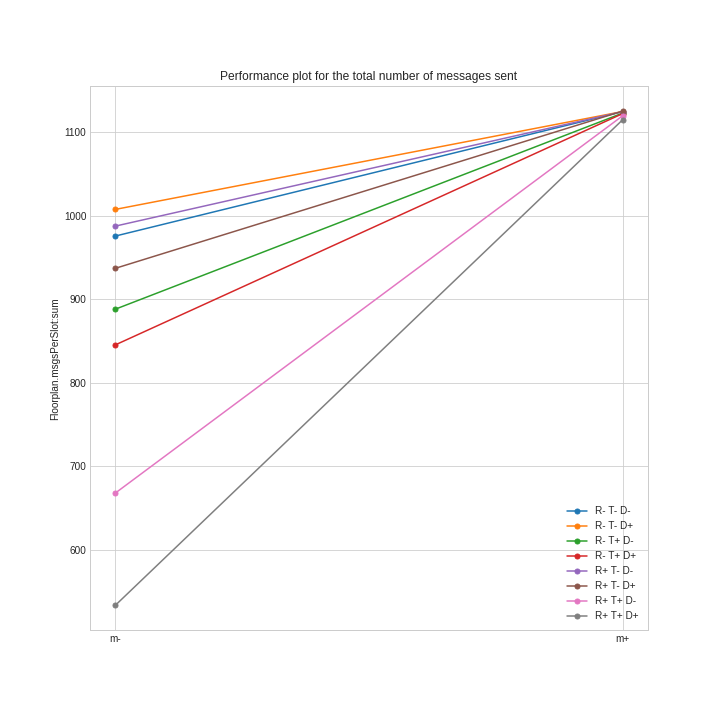
\includegraphics[width=\textwidth]{img/hd/messages-m-perfplot}
	\end{columns}
\end{frame}

\begin{frame}{High density (optimizations)}
	\begin{columns}
		\footnotesize
		\column{0.5\textwidth}
		\begin{itemize}
			\item Good coverage with \(R \ge 8m\)
			\item Broadcast time can be improved by increasing \(R\)
				(sacrifice energy efficiency) or by reducing
				\(T\)
		\end{itemize}
		\begin{center}
			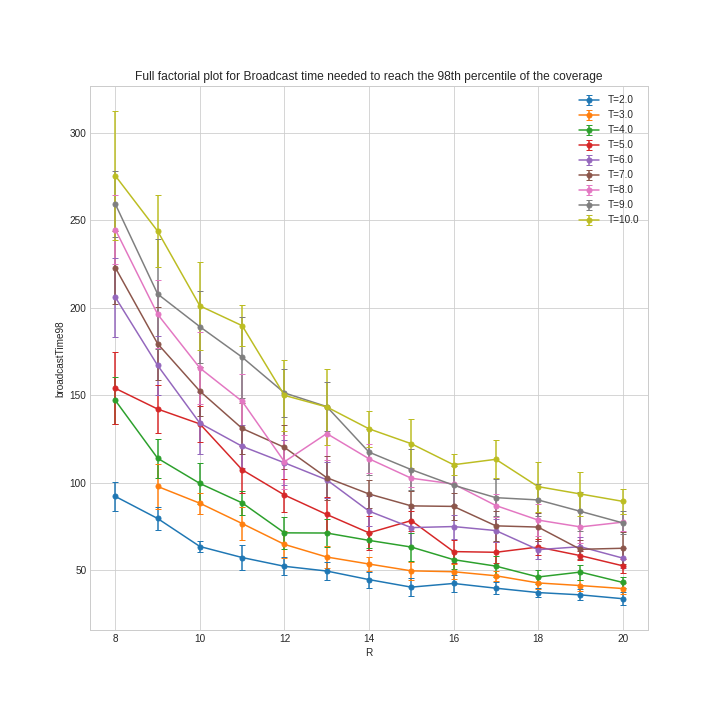
\includegraphics[width=0.8\textwidth]{img/hd/broadcasttime-R-ffplot}
		\end{center}
		\column{0.5\textwidth}
		\begin{itemize}
			\item Low \(m\) and high \(\max(\delta)\) reduce the
				number of collisions without sacrificing
				anything else
			\item Good linear relationship between collisions and
				\(\max(\delta)\)
		\end{itemize}
		\begin{center}
			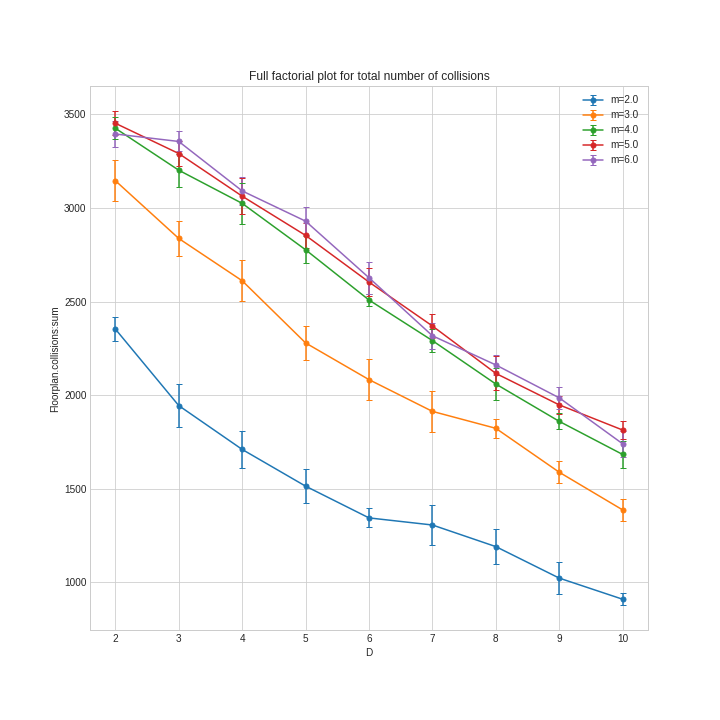
\includegraphics[width=0.75\textwidth]{img/hd/collisions-D-ffplot}
		\end{center}
	\end{columns}
\end{frame}

\begin{frame}{Low density (\(2^{k}r\))}
	\begin{columns}
		\column{0.5\textwidth}
		Also in this case the coverage always reach high values (\(> 99\%\))

		\begin{table}
			\begin{tabular}{l | c | c}
				Parameter & Factor & Percentage \\
				\hline \hline
				Collisions & R & \(58.96\%\) \\
				& m & \(19.26\%\) \\
				\hline
				Messages & m & \(85.18\%\) \\
				\hline
				Broadcast Time & R & \(58.90\%\) \\
				& T & \(30.43\%\) \\
				\hline
			\end{tabular}
			\caption{Most influencing factors for parameters}
		\end{table}
		\column{0.5\textwidth}
		\begin{figure}
		    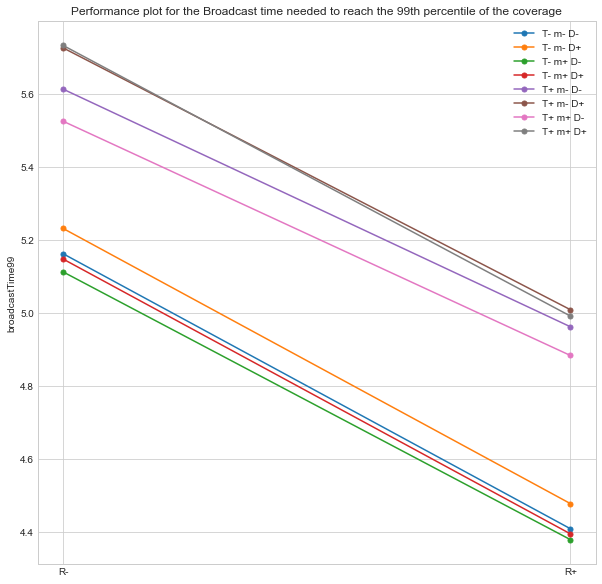
\includegraphics[height=0.65\textheight]{img/ld/broadcasttime-R-perfplot}
		    \caption{Increase R reduces so much the broadcast time (but increases the number of collisions and the energy consumed)}
		\end{figure}
	\end{columns}
\end{frame}

\begin{frame}{Low density (optimizations)}
	\footnotesize
	\begin{columns}
	    \column{0.5\textwidth}
	        \begin{itemize}
	        \item The minimum value of R to have a good coverage (\(> 99\%\)) is 25m
	        \item To improve energy efficiency, we should avoid to increase
			the broadcast radius (the hear window can be used
			instead)
	        \end{itemize}
	        \begin{center}
	            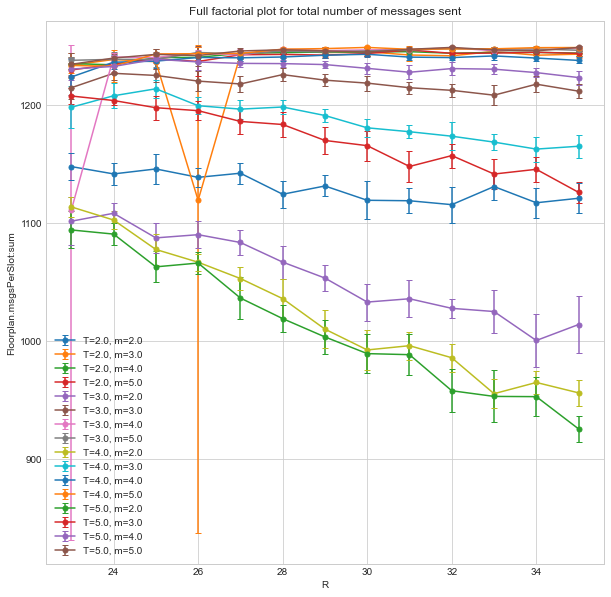
\includegraphics[width=0.7\textwidth]{img/ld/messages-R-ffplot.png}
	        \end{center}
	    \column{0.5\textwidth}
	        \begin{itemize}
	        \item A low number of max copies implies great benefits for all parameters
	        \item Trade-off between broadcast time and energy efficiency for the hear window parameter
	        \end{itemize}
	        \begin{center}
	            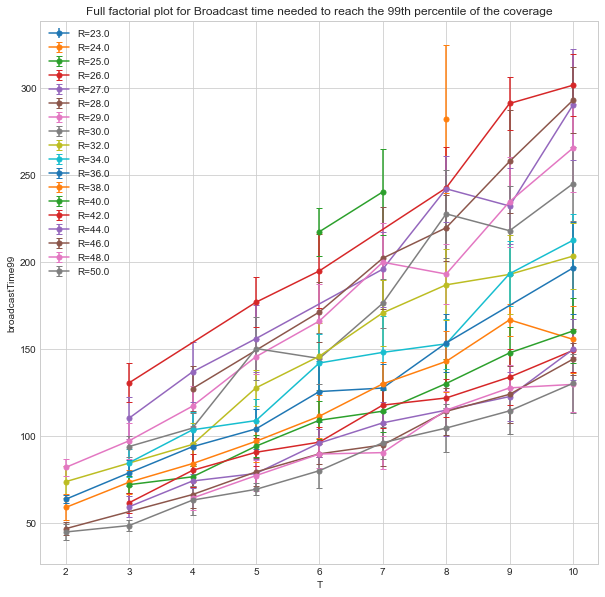
\includegraphics[width=0.7\textwidth]{img/ld/broadcasttime-T-ffplot.png}
	        \end{center}
	\end{columns}
\end{frame}

\begin{frame}{Rectangular floorplan}
		\begin{columns}
		\column{0.5\textwidth}
		 \begin{itemize}
		     \item
	Coverage almost always reaches 100\%.The lowest value is 99.6664\%. \\[5pt]

		\begin{table}
			\begin{tabular}{l | c | c}
				Parameter & Factor & Percentage \\
				\hline \hline
				Collisions & R & \(64.31 \%\) \\
				& m & \(16.47\%\) \\& Rm& \(9.59 \%\) \\
				\hline
				Messages & m & \(84.89\%\) \\& R & \(5.58\%\) \\
				\hline
				Broadcast Time & R & \(65.40\%\) \\
				& T & \(20.58\%\) \\
				\hline
			\end{tabular}
			\caption{Most influencing factors for parameters}
		\end{table}
		\item the shape of the plane has a negligible influence, so the obtained results for the optimizations are similar to previous ones
		\end{itemize}
		\column{0.5\textwidth}
				\begin{figure}
		    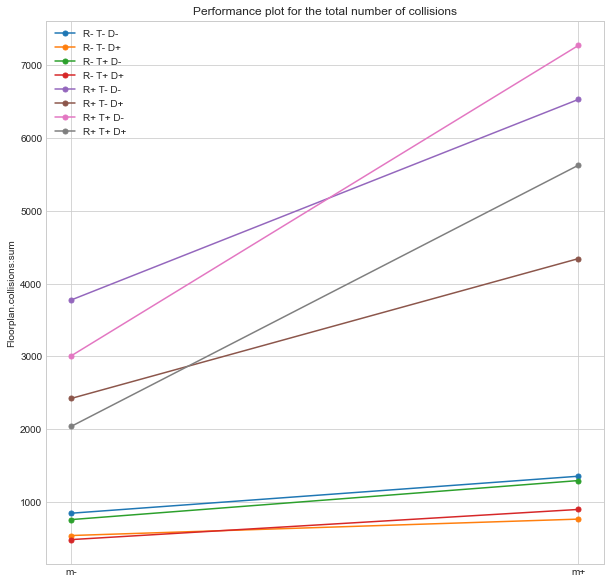
\includegraphics[height=0.65\textheight]{img/rect/collisions_m_perfplot.png}
		    \caption{Decrease the maximum number of copies to decrease the total
number of collisions}
		\end{figure}

	\end{columns}
\end{frame}

\begin{frame}{Position of starting node}
	\begin{columns}
		\column{0.5\textwidth}
		The broadcast time changes with the initial position of the
		first user. In the corner, the mean and the minimum broadcast
		time are lower than in the center.\\[10pt]
		\begin{tabular}{lcccc}
		\multicolumn{5}{c}{Low density (98th percentile broadcast time)}\\
		\toprule
		Start Node Pos\@. & Mean & Std\@. Dev\@. & Min\@. & Max\@. \\
		\midrule
		Center & \(35.166667s\) & \(1.533158s\) & \(31s\) & \(40s\) \\
		Border & \(53.7s\) & \(1.914554s\) & \(50s\) & \(58s\) \\
		Corner & \(65.1s\) & \(2.186952s\) & \(61s\) & \(70s\) \\
		\bottomrule
	    \end{tabular}
		\column{0.5\textwidth}
		    \begin{center}
		    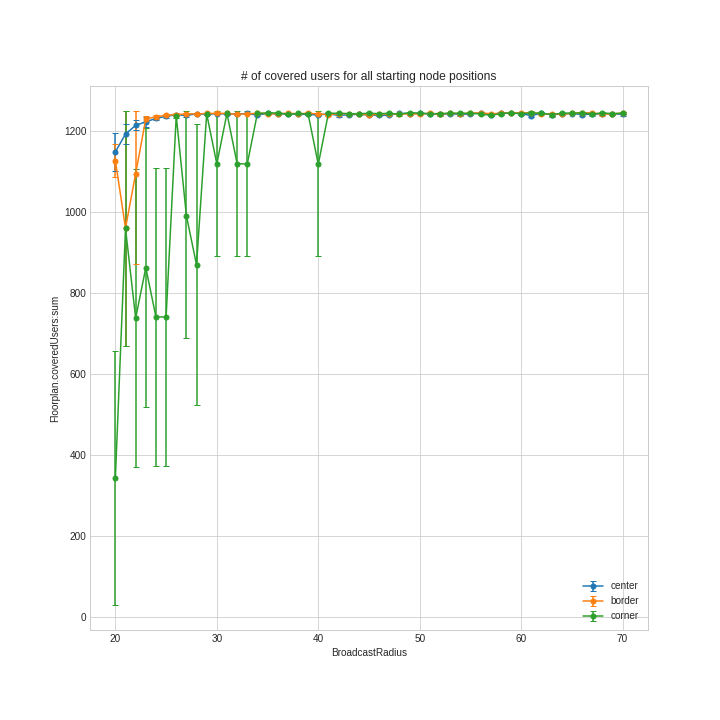
\includegraphics[height=0.7\textheight]{img/ld/start-node-coverage.png}
		    \end{center}
	\end{columns}
	The coverage drops down for low values of \(R\) when the position of the
	starting node is in the corner/border. In this points, we also have
	higher variance due to catastrophic situations where the network is not
	able to reach anyone
\end{frame}

\section{Conclusions}

\begin{frame}{Conclusions}
	\large
	\begin{itemize}
		\item Trade-off needed between broadcast time and energy
			efficiency on the \(R\) and \(T\) parameters
		\item Coverage almost always perfect with a good \(R\), except
			in some catastrophic cases when the starting node is in
			the corner. The probability to reach at least a user can
			be computed as:
			\[
				P = 1 - {\left(\frac{XY - \alpha\pi R^2}{XY}\right)}^{N-1}
			\]
		\item Trickle relaying is very effective to reduce collisions
			when using low \(m\)
		\item Shape of the floorplan generally irrelevant: slight
			increase in the broadcast time
		\item Position of the starting node, possibly in the center, is
			very important to have a good coverage and a low
			broadcast time
	\end{itemize}
\end{frame}

\begin{frame}
    \centering
    \Huge \color{blue} Thank you!
\end{frame}

\end{document}
